% Options for packages loaded elsewhere
\PassOptionsToPackage{unicode}{hyperref}
\PassOptionsToPackage{hyphens}{url}
\documentclass[
]{article}
\usepackage{xcolor}
\usepackage[margin=1in]{geometry}
\usepackage{amsmath,amssymb}
\setcounter{secnumdepth}{-\maxdimen} % remove section numbering
\usepackage{iftex}
\ifPDFTeX
  \usepackage[T1]{fontenc}
  \usepackage[utf8]{inputenc}
  \usepackage{textcomp} % provide euro and other symbols
\else % if luatex or xetex
  \usepackage{unicode-math} % this also loads fontspec
  \defaultfontfeatures{Scale=MatchLowercase}
  \defaultfontfeatures[\rmfamily]{Ligatures=TeX,Scale=1}
\fi
\usepackage{lmodern}
\ifPDFTeX\else
  % xetex/luatex font selection
\fi
% Use upquote if available, for straight quotes in verbatim environments
\IfFileExists{upquote.sty}{\usepackage{upquote}}{}
\IfFileExists{microtype.sty}{% use microtype if available
  \usepackage[]{microtype}
  \UseMicrotypeSet[protrusion]{basicmath} % disable protrusion for tt fonts
}{}
\makeatletter
\@ifundefined{KOMAClassName}{% if non-KOMA class
  \IfFileExists{parskip.sty}{%
    \usepackage{parskip}
  }{% else
    \setlength{\parindent}{0pt}
    \setlength{\parskip}{6pt plus 2pt minus 1pt}}
}{% if KOMA class
  \KOMAoptions{parskip=half}}
\makeatother
\usepackage{color}
\usepackage{fancyvrb}
\newcommand{\VerbBar}{|}
\newcommand{\VERB}{\Verb[commandchars=\\\{\}]}
\DefineVerbatimEnvironment{Highlighting}{Verbatim}{commandchars=\\\{\}}
% Add ',fontsize=\small' for more characters per line
\usepackage{framed}
\definecolor{shadecolor}{RGB}{248,248,248}
\newenvironment{Shaded}{\begin{snugshade}}{\end{snugshade}}
\newcommand{\AlertTok}[1]{\textcolor[rgb]{0.94,0.16,0.16}{#1}}
\newcommand{\AnnotationTok}[1]{\textcolor[rgb]{0.56,0.35,0.01}{\textbf{\textit{#1}}}}
\newcommand{\AttributeTok}[1]{\textcolor[rgb]{0.13,0.29,0.53}{#1}}
\newcommand{\BaseNTok}[1]{\textcolor[rgb]{0.00,0.00,0.81}{#1}}
\newcommand{\BuiltInTok}[1]{#1}
\newcommand{\CharTok}[1]{\textcolor[rgb]{0.31,0.60,0.02}{#1}}
\newcommand{\CommentTok}[1]{\textcolor[rgb]{0.56,0.35,0.01}{\textit{#1}}}
\newcommand{\CommentVarTok}[1]{\textcolor[rgb]{0.56,0.35,0.01}{\textbf{\textit{#1}}}}
\newcommand{\ConstantTok}[1]{\textcolor[rgb]{0.56,0.35,0.01}{#1}}
\newcommand{\ControlFlowTok}[1]{\textcolor[rgb]{0.13,0.29,0.53}{\textbf{#1}}}
\newcommand{\DataTypeTok}[1]{\textcolor[rgb]{0.13,0.29,0.53}{#1}}
\newcommand{\DecValTok}[1]{\textcolor[rgb]{0.00,0.00,0.81}{#1}}
\newcommand{\DocumentationTok}[1]{\textcolor[rgb]{0.56,0.35,0.01}{\textbf{\textit{#1}}}}
\newcommand{\ErrorTok}[1]{\textcolor[rgb]{0.64,0.00,0.00}{\textbf{#1}}}
\newcommand{\ExtensionTok}[1]{#1}
\newcommand{\FloatTok}[1]{\textcolor[rgb]{0.00,0.00,0.81}{#1}}
\newcommand{\FunctionTok}[1]{\textcolor[rgb]{0.13,0.29,0.53}{\textbf{#1}}}
\newcommand{\ImportTok}[1]{#1}
\newcommand{\InformationTok}[1]{\textcolor[rgb]{0.56,0.35,0.01}{\textbf{\textit{#1}}}}
\newcommand{\KeywordTok}[1]{\textcolor[rgb]{0.13,0.29,0.53}{\textbf{#1}}}
\newcommand{\NormalTok}[1]{#1}
\newcommand{\OperatorTok}[1]{\textcolor[rgb]{0.81,0.36,0.00}{\textbf{#1}}}
\newcommand{\OtherTok}[1]{\textcolor[rgb]{0.56,0.35,0.01}{#1}}
\newcommand{\PreprocessorTok}[1]{\textcolor[rgb]{0.56,0.35,0.01}{\textit{#1}}}
\newcommand{\RegionMarkerTok}[1]{#1}
\newcommand{\SpecialCharTok}[1]{\textcolor[rgb]{0.81,0.36,0.00}{\textbf{#1}}}
\newcommand{\SpecialStringTok}[1]{\textcolor[rgb]{0.31,0.60,0.02}{#1}}
\newcommand{\StringTok}[1]{\textcolor[rgb]{0.31,0.60,0.02}{#1}}
\newcommand{\VariableTok}[1]{\textcolor[rgb]{0.00,0.00,0.00}{#1}}
\newcommand{\VerbatimStringTok}[1]{\textcolor[rgb]{0.31,0.60,0.02}{#1}}
\newcommand{\WarningTok}[1]{\textcolor[rgb]{0.56,0.35,0.01}{\textbf{\textit{#1}}}}
\usepackage{graphicx}
\makeatletter
\newsavebox\pandoc@box
\newcommand*\pandocbounded[1]{% scales image to fit in text height/width
  \sbox\pandoc@box{#1}%
  \Gscale@div\@tempa{\textheight}{\dimexpr\ht\pandoc@box+\dp\pandoc@box\relax}%
  \Gscale@div\@tempb{\linewidth}{\wd\pandoc@box}%
  \ifdim\@tempb\p@<\@tempa\p@\let\@tempa\@tempb\fi% select the smaller of both
  \ifdim\@tempa\p@<\p@\scalebox{\@tempa}{\usebox\pandoc@box}%
  \else\usebox{\pandoc@box}%
  \fi%
}
% Set default figure placement to htbp
\def\fps@figure{htbp}
\makeatother
\setlength{\emergencystretch}{3em} % prevent overfull lines
\providecommand{\tightlist}{%
  \setlength{\itemsep}{0pt}\setlength{\parskip}{0pt}}
\usepackage{bookmark}
\IfFileExists{xurl.sty}{\usepackage{xurl}}{} % add URL line breaks if available
\urlstyle{same}
\hypersetup{
  pdftitle={Inference for categorical data},
  hidelinks,
  pdfcreator={LaTeX via pandoc}}

\title{Inference for categorical data}
\author{}
\date{\vspace{-2.5em}}

\begin{document}
\maketitle

\subsection{Getting Started}\label{getting-started}

\subsubsection{Load packages}\label{load-packages}

In this lab, we will explore and visualize the data using the
\textbf{tidyverse} suite of packages, and perform statistical inference
using \textbf{infer}. The data can be found in the companion package for
OpenIntro resources, \textbf{openintro}.

Let's load the packages.

\begin{Shaded}
\begin{Highlighting}[]
\FunctionTok{library}\NormalTok{(tidyverse)}
\FunctionTok{library}\NormalTok{(openintro)}
\FunctionTok{library}\NormalTok{(infer)}
\end{Highlighting}
\end{Shaded}

\begin{Shaded}
\begin{Highlighting}[]
\FunctionTok{options}\NormalTok{(}\AttributeTok{tibble.width =} \ConstantTok{Inf}\NormalTok{)}
\end{Highlighting}
\end{Shaded}

\subsubsection{The data}\label{the-data}

You will be analyzing the same dataset as in the previous lab, where you
delved into a sample from the Youth Risk Behavior Surveillance System
(YRBSS) survey, which uses data from high schoolers to help discover
health patterns. The dataset is called \texttt{yrbss}.

\begin{enumerate}
\def\labelenumi{\arabic{enumi}.}
\tightlist
\item
  What are the counts within each category for the amount of days these
  students have texted while driving within the past 30 days?
\end{enumerate}

\textbf{Insert your answer here}

\begin{Shaded}
\begin{Highlighting}[]
\FunctionTok{view}\NormalTok{(yrbss)}
\end{Highlighting}
\end{Shaded}

\begin{Shaded}
\begin{Highlighting}[]
\NormalTok{yrbss }\SpecialCharTok{\%\textgreater{}\%}
  \FunctionTok{count}\NormalTok{(text\_while\_driving\_30d)}
\end{Highlighting}
\end{Shaded}

\begin{verbatim}
## # A tibble: 9 x 2
##   text_while_driving_30d     n
##   <chr>                  <int>
## 1 0                       4792
## 2 1-2                      925
## 3 10-19                    373
## 4 20-29                    298
## 5 3-5                      493
## 6 30                       827
## 7 6-9                      311
## 8 did not drive           4646
## 9 <NA>                     918
\end{verbatim}

Among the 13,583 students: 0 days = 4,792, 1-2 days = 925, 3-5 days =
493, 6-9 days = 311, 10-19 days = 373, 20-29 days = 298, all 30 days =
827, did not drive = 4,646, missing = 918.

\begin{enumerate}
\def\labelenumi{\arabic{enumi}.}
\setcounter{enumi}{1}
\tightlist
\item
  What is the proportion of people who have texted while driving every
  day in the past 30 days and never wear helmets?
\end{enumerate}

\textbf{Insert your answer here}

\begin{Shaded}
\begin{Highlighting}[]
\NormalTok{yrbss }\SpecialCharTok{\%\textgreater{}\%}
  \FunctionTok{filter}\NormalTok{(helmet\_12m }\SpecialCharTok{==} \StringTok{"never"}\NormalTok{) }\SpecialCharTok{\%\textgreater{}\%}
  \FunctionTok{mutate}\NormalTok{(}\AttributeTok{text\_ind =} \FunctionTok{ifelse}\NormalTok{(text\_while\_driving\_30d }\SpecialCharTok{==} \StringTok{"30"}\NormalTok{, }\StringTok{"yes"}\NormalTok{, }\StringTok{"no"}\NormalTok{)) }\SpecialCharTok{\%\textgreater{}\%}
  \FunctionTok{drop\_na}\NormalTok{(text\_ind) }\SpecialCharTok{\%\textgreater{}\%}
  \FunctionTok{count}\NormalTok{(text\_ind) }\SpecialCharTok{\%\textgreater{}\%}
  \FunctionTok{mutate}\NormalTok{(}\AttributeTok{prop =}\NormalTok{ n }\SpecialCharTok{/} \FunctionTok{sum}\NormalTok{(n))}
\end{Highlighting}
\end{Shaded}

\begin{verbatim}
## # A tibble: 2 x 3
##   text_ind     n   prop
##   <chr>    <int>  <dbl>
## 1 no        6040 0.929 
## 2 yes        463 0.0712
\end{verbatim}

Among non-helmet wearers with a response, 463 of 6,503 texted while
driving every day, so the proportion is about 0.071\textbf{.}

Remember that you can use \texttt{filter} to limit the dataset to just
non-helmet wearers. Here, we will name the dataset \texttt{no\_helmet}.

\begin{Shaded}
\begin{Highlighting}[]
\FunctionTok{data}\NormalTok{(}\StringTok{\textquotesingle{}yrbss\textquotesingle{}}\NormalTok{, }\AttributeTok{package=}\StringTok{\textquotesingle{}openintro\textquotesingle{}}\NormalTok{)}
\NormalTok{no\_helmet }\OtherTok{\textless{}{-}}\NormalTok{ yrbss }\SpecialCharTok{\%\textgreater{}\%}
  \FunctionTok{filter}\NormalTok{(helmet\_12m }\SpecialCharTok{==} \StringTok{"never"}\NormalTok{)}
\end{Highlighting}
\end{Shaded}

Also, it may be easier to calculate the proportion if you create a new
variable that specifies whether the individual has texted every day
while driving over the past 30 days or not. We will call this variable
\texttt{text\_ind}.

\begin{Shaded}
\begin{Highlighting}[]
\NormalTok{no\_helmet }\OtherTok{\textless{}{-}}\NormalTok{ no\_helmet }\SpecialCharTok{\%\textgreater{}\%}
  \FunctionTok{mutate}\NormalTok{(}\AttributeTok{text\_ind =} \FunctionTok{ifelse}\NormalTok{(text\_while\_driving\_30d }\SpecialCharTok{==} \StringTok{"30"}\NormalTok{, }\StringTok{"yes"}\NormalTok{, }\StringTok{"no"}\NormalTok{))}
\end{Highlighting}
\end{Shaded}

\subsection{Inference on proportions}\label{inference-on-proportions}

When summarizing the YRBSS, the Centers for Disease Control and
Prevention seeks insight into the population \emph{parameters}. To do
this, you can answer the question, ``What proportion of people in your
sample reported that they have texted while driving each day for the
past 30 days?'' with a statistic; while the question ``What proportion
of people on earth have texted while driving each day for the past 30
days?'' is answered with an estimate of the parameter.

The inferential tools for estimating population proportion are analogous
to those used for means in the last chapter: the confidence interval and
the hypothesis test.

\begin{Shaded}
\begin{Highlighting}[]
\NormalTok{no\_helmet }\SpecialCharTok{\%\textgreater{}\%}
  \FunctionTok{drop\_na}\NormalTok{(text\_ind) }\SpecialCharTok{\%\textgreater{}\%} \CommentTok{\# Drop missing values}
  \FunctionTok{specify}\NormalTok{(}\AttributeTok{response =}\NormalTok{ text\_ind, }\AttributeTok{success =} \StringTok{"yes"}\NormalTok{) }\SpecialCharTok{\%\textgreater{}\%}
  \FunctionTok{generate}\NormalTok{(}\AttributeTok{reps =} \DecValTok{1000}\NormalTok{, }\AttributeTok{type =} \StringTok{"bootstrap"}\NormalTok{) }\SpecialCharTok{\%\textgreater{}\%}
  \FunctionTok{calculate}\NormalTok{(}\AttributeTok{stat =} \StringTok{"prop"}\NormalTok{) }\SpecialCharTok{\%\textgreater{}\%}
  \FunctionTok{get\_ci}\NormalTok{(}\AttributeTok{level =} \FloatTok{0.95}\NormalTok{)}
\end{Highlighting}
\end{Shaded}

\begin{verbatim}
## # A tibble: 1 x 2
##   lower_ci upper_ci
##      <dbl>    <dbl>
## 1   0.0652   0.0777
\end{verbatim}

Note that since the goal is to construct an interval estimate for a
proportion, it's necessary to both include the \texttt{success} argument
within \texttt{specify}, which accounts for the proportion of non-helmet
wearers than have consistently texted while driving the past 30 days, in
this example, and that \texttt{stat} within \texttt{calculate} is here
``prop'', signaling that you are trying to do some sort of inference on
a proportion.

\begin{enumerate}
\def\labelenumi{\arabic{enumi}.}
\setcounter{enumi}{2}
\tightlist
\item
  What is the margin of error for the estimate of the proportion of
  non-helmet wearers that have texted while driving each day for the
  past 30 days based on this survey?
\end{enumerate}

\textbf{Insert your answer here}

\begin{Shaded}
\begin{Highlighting}[]
\FunctionTok{set.seed}\NormalTok{(}\DecValTok{607}\NormalTok{)}
\NormalTok{nohelmet\_ci }\OtherTok{\textless{}{-}}\NormalTok{ no\_helmet }\SpecialCharTok{\%\textgreater{}\%}
  \FunctionTok{drop\_na}\NormalTok{(text\_ind) }\SpecialCharTok{\%\textgreater{}\%}
  \FunctionTok{specify}\NormalTok{(}\AttributeTok{response =}\NormalTok{ text\_ind, }\AttributeTok{success =} \StringTok{"yes"}\NormalTok{) }\SpecialCharTok{\%\textgreater{}\%}
  \FunctionTok{generate}\NormalTok{(}\AttributeTok{reps =} \DecValTok{1000}\NormalTok{, }\AttributeTok{type =} \StringTok{"bootstrap"}\NormalTok{) }\SpecialCharTok{\%\textgreater{}\%}
  \FunctionTok{calculate}\NormalTok{(}\AttributeTok{stat =} \StringTok{"prop"}\NormalTok{) }\SpecialCharTok{\%\textgreater{}\%}
  \FunctionTok{get\_ci}\NormalTok{(}\AttributeTok{level =} \FloatTok{0.95}\NormalTok{)}

\NormalTok{nohelmet\_ci}
\end{Highlighting}
\end{Shaded}

\begin{verbatim}
## # A tibble: 1 x 2
##   lower_ci upper_ci
##      <dbl>    <dbl>
## 1   0.0650   0.0773
\end{verbatim}

\begin{Shaded}
\begin{Highlighting}[]
\NormalTok{(nohelmet\_ci}\SpecialCharTok{$}\NormalTok{upper\_ci }\SpecialCharTok{{-}}\NormalTok{ nohelmet\_ci}\SpecialCharTok{$}\NormalTok{lower\_ci) }\SpecialCharTok{/} \DecValTok{2}
\end{Highlighting}
\end{Shaded}

\begin{verbatim}
## [1] 0.006151007
\end{verbatim}

The 95\% interval is roughly (0.065, 0.078), so the margin of error is
about 0.006.

\begin{enumerate}
\def\labelenumi{\arabic{enumi}.}
\setcounter{enumi}{3}
\tightlist
\item
  Using the \texttt{infer} package, calculate confidence intervals for
  two other categorical variables (you'll need to decide which level to
  call ``success'', and report the associated margins of error. Interpet
  the interval in context of the data. It may be helpful to create new
  data sets for each of the two countries first, and then use these data
  sets to construct the confidence intervals.
\end{enumerate}

\textbf{Insert your answer here}

I chose the proportion of students who are Hispanic and the proportion
who sleep fewer than 5 hours on school nights.

\begin{Shaded}
\begin{Highlighting}[]
\NormalTok{hispanic\_ci }\OtherTok{\textless{}{-}}\NormalTok{ yrbss }\SpecialCharTok{\%\textgreater{}\%}
  \FunctionTok{drop\_na}\NormalTok{(hispanic) }\SpecialCharTok{\%\textgreater{}\%}
  \FunctionTok{specify}\NormalTok{(}\AttributeTok{response =}\NormalTok{ hispanic, }\AttributeTok{success =} \StringTok{"hispanic"}\NormalTok{) }\SpecialCharTok{\%\textgreater{}\%}
  \FunctionTok{generate}\NormalTok{(}\AttributeTok{reps =} \DecValTok{1000}\NormalTok{, }\AttributeTok{type =} \StringTok{"bootstrap"}\NormalTok{) }\SpecialCharTok{\%\textgreater{}\%}
  \FunctionTok{calculate}\NormalTok{(}\AttributeTok{stat =} \StringTok{"prop"}\NormalTok{) }\SpecialCharTok{\%\textgreater{}\%}
  \FunctionTok{get\_ci}\NormalTok{(}\AttributeTok{level =} \FloatTok{0.95}\NormalTok{)}

\NormalTok{sleep5\_ci }\OtherTok{\textless{}{-}}\NormalTok{ yrbss }\SpecialCharTok{\%\textgreater{}\%}
  \FunctionTok{drop\_na}\NormalTok{(school\_night\_hours\_sleep) }\SpecialCharTok{\%\textgreater{}\%}
  \FunctionTok{mutate}\NormalTok{(}\AttributeTok{sleep\_lt5 =} \FunctionTok{ifelse}\NormalTok{(school\_night\_hours\_sleep }\SpecialCharTok{==} \StringTok{"\textless{}5"}\NormalTok{, }\StringTok{"yes"}\NormalTok{, }\StringTok{"no"}\NormalTok{)) }\SpecialCharTok{\%\textgreater{}\%}
  \FunctionTok{specify}\NormalTok{(}\AttributeTok{response =}\NormalTok{ sleep\_lt5, }\AttributeTok{success =} \StringTok{"yes"}\NormalTok{) }\SpecialCharTok{\%\textgreater{}\%}
  \FunctionTok{generate}\NormalTok{(}\AttributeTok{reps =} \DecValTok{1000}\NormalTok{, }\AttributeTok{type =} \StringTok{"bootstrap"}\NormalTok{) }\SpecialCharTok{\%\textgreater{}\%}
  \FunctionTok{calculate}\NormalTok{(}\AttributeTok{stat =} \StringTok{"prop"}\NormalTok{) }\SpecialCharTok{\%\textgreater{}\%}
  \FunctionTok{get\_ci}\NormalTok{(}\AttributeTok{level =} \FloatTok{0.95}\NormalTok{)}

\FunctionTok{bind\_rows}\NormalTok{(}\AttributeTok{hispanic =}\NormalTok{ hispanic\_ci, }\AttributeTok{sleep\_lt5 =}\NormalTok{ sleep5\_ci, }\AttributeTok{.id =} \StringTok{"variable"}\NormalTok{) }\SpecialCharTok{\%\textgreater{}\%}
  \FunctionTok{mutate}\NormalTok{(}\AttributeTok{margin\_of\_error =}\NormalTok{ (upper\_ci }\SpecialCharTok{{-}}\NormalTok{ lower\_ci) }\SpecialCharTok{/} \DecValTok{2}\NormalTok{)}
\end{Highlighting}
\end{Shaded}

\begin{verbatim}
## # A tibble: 2 x 4
##   variable  lower_ci upper_ci margin_of_error
##   <chr>        <dbl>    <dbl>           <dbl>
## 1 hispanic    0.249    0.264          0.00772
## 2 sleep_lt5   0.0738   0.0831         0.00466
\end{verbatim}

Hispanic (success = ``hispanic''): \(\hat{p} \approx 0.256\), 95\% CI
margin of error about 0.007. We are 95\% confident that between about
24.9\% and 26.4\% of the high schoolers in the population this survey
represents are Hispanic. Sleeps \textless{} 5 hours on school nights
(success = ``\textless5''): \(\hat{p} \approx 0.078\), 95\% CI margin of
error about 0.005. We are 95\% confident that between about 7.3\% and
8.3\% of these high schoolers sleep fewer than 5 hours on school nights.

The second interval is narrower because \(p\) is closer to 0, which
gives a smaller \(p(1-p)\).

\subsection{How does the proportion affect the margin of
error?}\label{how-does-the-proportion-affect-the-margin-of-error}

Imagine you've set out to survey 1000 people on two questions: are you
at least 6-feet tall? and are you left-handed? Since both of these
sample proportions were calculated from the same sample size, they
should have the same margin of error, right? Wrong! While the margin of
error does change with sample size, it is also affected by the
proportion.

Think back to the formula for the standard error:
\(SE = \sqrt{p(1-p)/n}\). This is then used in the formula for the
margin of error for a 95\% confidence interval:

\[ME = 1.96\times SE = 1.96\times\sqrt{p(1-p)/n} \,.\] Since the
population proportion \(p\) is in this \(ME\) formula, it should make
sense that the margin of error is in some way dependent on the
population proportion. We can visualize this relationship by creating a
plot of \(ME\) vs.~\(p\).

Since sample size is irrelevant to this discussion, let's just set it to
some value (\(n = 1000\)) and use this value in the following
calculations:

\begin{Shaded}
\begin{Highlighting}[]
\NormalTok{n }\OtherTok{\textless{}{-}} \DecValTok{1000}
\end{Highlighting}
\end{Shaded}

The first step is to make a variable \texttt{p} that is a sequence from
0 to 1 with each number incremented by 0.01. You can then create a
variable of the margin of error (\texttt{me}) associated with each of
these values of \texttt{p} using the familiar approximate formula
(\(ME = 2 \times SE\)).

\begin{Shaded}
\begin{Highlighting}[]
\NormalTok{p }\OtherTok{\textless{}{-}} \FunctionTok{seq}\NormalTok{(}\AttributeTok{from =} \DecValTok{0}\NormalTok{, }\AttributeTok{to =} \DecValTok{1}\NormalTok{, }\AttributeTok{by =} \FloatTok{0.01}\NormalTok{)}
\NormalTok{me }\OtherTok{\textless{}{-}} \DecValTok{2} \SpecialCharTok{*} \FunctionTok{sqrt}\NormalTok{(p }\SpecialCharTok{*}\NormalTok{ (}\DecValTok{1} \SpecialCharTok{{-}}\NormalTok{ p)}\SpecialCharTok{/}\NormalTok{n)}
\end{Highlighting}
\end{Shaded}

Lastly, you can plot the two variables against each other to reveal
their relationship. To do so, we need to first put these variables in a
data frame that you can call in the \texttt{ggplot} function.

\begin{Shaded}
\begin{Highlighting}[]
\NormalTok{dd }\OtherTok{\textless{}{-}} \FunctionTok{data.frame}\NormalTok{(}\AttributeTok{p =}\NormalTok{ p, }\AttributeTok{me =}\NormalTok{ me)}
\FunctionTok{ggplot}\NormalTok{(}\AttributeTok{data =}\NormalTok{ dd, }\FunctionTok{aes}\NormalTok{(}\AttributeTok{x =}\NormalTok{ p, }\AttributeTok{y =}\NormalTok{ me)) }\SpecialCharTok{+} 
  \FunctionTok{geom\_line}\NormalTok{() }\SpecialCharTok{+}
  \FunctionTok{labs}\NormalTok{(}\AttributeTok{x =} \StringTok{"Population Proportion"}\NormalTok{, }\AttributeTok{y =} \StringTok{"Margin of Error"}\NormalTok{)}
\end{Highlighting}
\end{Shaded}

\pandocbounded{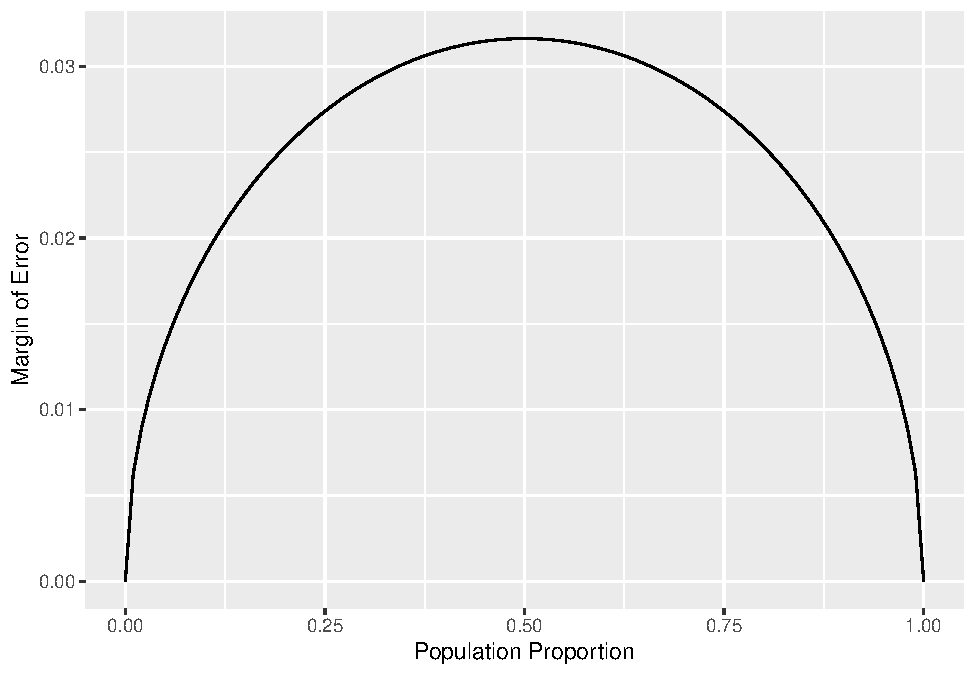
\includegraphics[keepaspectratio]{Lab6_inf_for_categorical_data_files/figure-latex/me-plot-1.pdf}}

\begin{enumerate}
\def\labelenumi{\arabic{enumi}.}
\setcounter{enumi}{4}
\tightlist
\item
  Describe the relationship between \texttt{p} and \texttt{me}. Include
  the margin of error vs.~population proportion plot you constructed in
  your answer. For a given sample size, for which value of \texttt{p} is
  margin of error maximized?
\end{enumerate}

\textbf{Insert your answer here}

The relationship is a symmetric, inverted-U (parabola-like) curve. The
margin of error is 0 at \(p = 0\) and \(p = 1\), rises as \(p\) moves
toward the middle, and is largest at \(p = 0.5\), where \(p(1-p)\) is
maximized. So for a fixed sample size, proportions near 0.5 are
estimated least precisely and proportions near 0 or 1 most precisely.

\subsection{Success-failure condition}\label{success-failure-condition}

We have emphasized that you must always check conditions before making
inference. For inference on proportions, the sample proportion can be
assumed to be nearly normal if it is based upon a random sample of
independent observations and if both \(np \geq 10\) and
\(n(1 - p) \geq 10\). This rule of thumb is easy enough to follow, but
it makes you wonder: what's so special about the number 10?

The short answer is: nothing. You could argue that you would be fine
with 9 or that you really should be using 11. What is the ``best'' value
for such a rule of thumb is, at least to some degree, arbitrary.
However, when \(np\) and \(n(1-p)\) reaches 10 the sampling distribution
is sufficiently normal to use confidence intervals and hypothesis tests
that are based on that approximation.

You can investigate the interplay between \(n\) and \(p\) and the shape
of the sampling distribution by using simulations. Play around with the
following app to investigate how the shape, center, and spread of the
distribution of \(\hat{p}\) changes as \(n\) and \(p\) changes.

\begin{enumerate}
\def\labelenumi{\arabic{enumi}.}
\setcounter{enumi}{5}
\tightlist
\item
  Describe the sampling distribution of sample proportions at
  \(n = 300\) and \(p = 0.1\). Be sure to note the center, spread, and
  shape.
\end{enumerate}

\textbf{Insert your answer here}

\pandocbounded{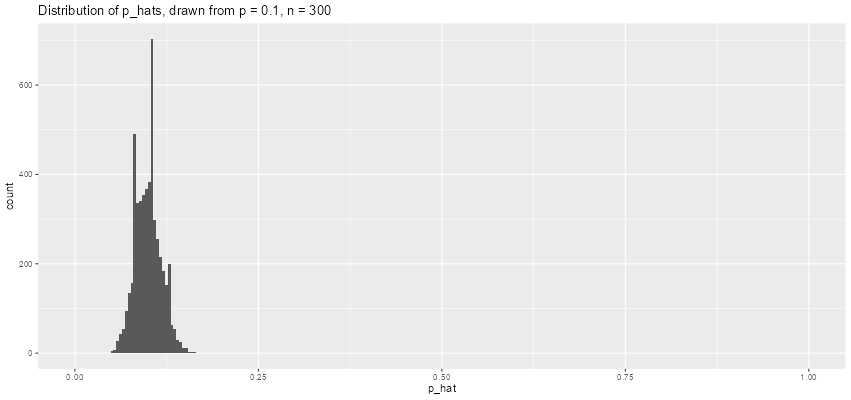
\includegraphics[keepaspectratio]{images/clipboard-2105274727.png}}

The center is at around 0.10. The spread seems to be somewhere around
0.06 and 0.14. It looks like a unimodal shape.

\begin{enumerate}
\def\labelenumi{\arabic{enumi}.}
\setcounter{enumi}{6}
\tightlist
\item
  Keep \(n\) constant and change \(p\). How does the shape, center, and
  spread of the sampling distribution vary as \(p\) changes. You might
  want to adjust min and max for the \(x\)-axis for a better view of the
  distribution.
\end{enumerate}

\textbf{Insert your answer here}

With n fixed at 300, the sampling distribution is always centered at
about p, so it slides along the x-axis as p changes. The spread is
largest at p = 0.5 and shrinks as p approaches 0 or 1. Near p = 0.5 the
shape is symmetric and approximately normal. As p gets small, the
distribution becomes right-skewed and is truncated at 0, and as p gets
large it becomes left-skewed.

\begin{enumerate}
\def\labelenumi{\arabic{enumi}.}
\setcounter{enumi}{7}
\tightlist
\item
  Now also change \(n\). How does \(n\) appear to affect the
  distribution of \(\hat{p}\)?
\end{enumerate}

\textbf{Insert your answer here}

The center stays at \(p\), but increasing \(n\) makes the distribution
narrower. A larger \(n\) also makes the shape more symmetric and normal,
because \(np\) and \(n(1-p)\) grow. A small \(n\) produces a wider,
lumpier, skewed distribution, especially when \(p\) is near 0 or 1.

\begin{center}\rule{0.5\linewidth}{0.5pt}\end{center}

\subsection{More Practice}\label{more-practice}

For some of the exercises below, you will conduct inference comparing
two proportions. In such cases, you have a response variable that is
categorical, and an explanatory variable that is also categorical, and
you are comparing the proportions of success of the response variable
across the levels of the explanatory variable. This means that when
using \texttt{infer}, you need to include both variables within
\texttt{specify}.

\begin{enumerate}
\def\labelenumi{\arabic{enumi}.}
\setcounter{enumi}{8}
\tightlist
\item
  Is there convincing evidence that those who sleep 10+ hours per day
  are more likely to strength train every day of the week? As always,
  write out the hypotheses for any tests you conduct and outline the
  status of the conditions for inference. If you find a significant
  difference, also quantify this difference with a confidence interval.
\end{enumerate}

\textbf{Insert your answer here}

Hypotheses: Let \(p_{10+}\) be the proportion of students sleeping 10+
hours who strength train all 7 days, and \(p_{<10}\) the proportion
among students sleeping fewer than 10 hours.

\begin{itemize}
\tightlist
\item
  \(H_0: p_{10+} = p_{<10}\) sleep is unrelated to training every day
\item
  \(H_A: p_{10+} > p_{<10}\) 10+ hour sleepers are more likely to train
  every day
\end{itemize}

\begin{Shaded}
\begin{Highlighting}[]
\NormalTok{sleep\_strength }\OtherTok{\textless{}{-}}\NormalTok{ yrbss }\SpecialCharTok{\%\textgreater{}\%}
  \FunctionTok{drop\_na}\NormalTok{(school\_night\_hours\_sleep, strength\_training\_7d) }\SpecialCharTok{\%\textgreater{}\%}
  \FunctionTok{mutate}\NormalTok{(}\AttributeTok{sleep\_10 =} \FunctionTok{ifelse}\NormalTok{(school\_night\_hours\_sleep }\SpecialCharTok{==} \StringTok{"10+"}\NormalTok{, }\StringTok{"10+"}\NormalTok{, }\StringTok{"\textless{}10"}\NormalTok{),}
         \AttributeTok{strength\_ind =} \FunctionTok{ifelse}\NormalTok{(strength\_training\_7d }\SpecialCharTok{==} \DecValTok{7}\NormalTok{, }\StringTok{"yes"}\NormalTok{, }\StringTok{"no"}\NormalTok{))}
\end{Highlighting}
\end{Shaded}

\begin{Shaded}
\begin{Highlighting}[]
\NormalTok{sleep\_strength }\SpecialCharTok{\%\textgreater{}\%}
  \FunctionTok{count}\NormalTok{(sleep\_10, strength\_ind)}
\end{Highlighting}
\end{Shaded}

\begin{verbatim}
## # A tibble: 4 x 3
##   sleep_10 strength_ind     n
##   <chr>    <chr>        <int>
## 1 10+      no             228
## 2 10+      yes             84
## 3 <10      no            9949
## 4 <10      yes           1958
\end{verbatim}

\begin{Shaded}
\begin{Highlighting}[]
\NormalTok{obs\_diff }\OtherTok{\textless{}{-}}\NormalTok{ sleep\_strength }\SpecialCharTok{\%\textgreater{}\%}
  \FunctionTok{specify}\NormalTok{(strength\_ind }\SpecialCharTok{\textasciitilde{}}\NormalTok{ sleep\_10, }\AttributeTok{success =} \StringTok{"yes"}\NormalTok{) }\SpecialCharTok{\%\textgreater{}\%}
  \FunctionTok{calculate}\NormalTok{(}\AttributeTok{stat =} \StringTok{"diff in props"}\NormalTok{, }\AttributeTok{order =} \FunctionTok{c}\NormalTok{(}\StringTok{"10+"}\NormalTok{, }\StringTok{"\textless{}10"}\NormalTok{))}
\end{Highlighting}
\end{Shaded}

\begin{Shaded}
\begin{Highlighting}[]
\FunctionTok{set.seed}\NormalTok{(}\DecValTok{607}\NormalTok{)}
\NormalTok{null\_dist }\OtherTok{\textless{}{-}}\NormalTok{ sleep\_strength }\SpecialCharTok{\%\textgreater{}\%}
  \FunctionTok{specify}\NormalTok{(strength\_ind }\SpecialCharTok{\textasciitilde{}}\NormalTok{ sleep\_10, }\AttributeTok{success =} \StringTok{"yes"}\NormalTok{) }\SpecialCharTok{\%\textgreater{}\%}
  \FunctionTok{hypothesize}\NormalTok{(}\AttributeTok{null =} \StringTok{"independence"}\NormalTok{) }\SpecialCharTok{\%\textgreater{}\%}
  \FunctionTok{generate}\NormalTok{(}\AttributeTok{reps =} \DecValTok{1000}\NormalTok{, }\AttributeTok{type =} \StringTok{"permute"}\NormalTok{) }\SpecialCharTok{\%\textgreater{}\%}
  \FunctionTok{calculate}\NormalTok{(}\AttributeTok{stat =} \StringTok{"diff in props"}\NormalTok{, }\AttributeTok{order =} \FunctionTok{c}\NormalTok{(}\StringTok{"10+"}\NormalTok{, }\StringTok{"\textless{}10"}\NormalTok{))}

\NormalTok{obs\_diff}
\end{Highlighting}
\end{Shaded}

\begin{verbatim}
## Response: strength_ind (factor)
## Explanatory: sleep_10 (factor)
## # A tibble: 1 x 1
##    stat
##   <dbl>
## 1 0.105
\end{verbatim}

\begin{Shaded}
\begin{Highlighting}[]
\NormalTok{null\_dist }\SpecialCharTok{\%\textgreater{}\%} \FunctionTok{get\_p\_value}\NormalTok{(}\AttributeTok{obs\_stat =}\NormalTok{ obs\_diff, }\AttributeTok{direction =} \StringTok{"greater"}\NormalTok{)}
\end{Highlighting}
\end{Shaded}

\begin{verbatim}
## # A tibble: 1 x 1
##   p_value
##     <dbl>
## 1       0
\end{verbatim}

Conditions: The YRBSS is a random sample well under 10\% of all U.S.
high schoolers, and the two groups are separate students, so
independence holds. With a pooled proportion of about 0.167, all
expected counts (about 52, 260, 1,990 and 9,917) are well above 10, so
the success-failure condition holds.

Result: 26.9\% of students sleeping 10+ hours, 84 of 312, strength train
all 7 days, versus 16.4\% of those sleeping less, 1,958 of 11,907, a
difference of about 0.105. No permuted difference came close, so p
\textless{} 0.001 (z ≈ 4.9). We reject H₀: there is convincing evidence
that students who sleep 10+ hours are more likely to strength train
every day.

\begin{Shaded}
\begin{Highlighting}[]
\FunctionTok{set.seed}\NormalTok{(}\DecValTok{607}\NormalTok{)}
\NormalTok{sleep\_strength }\SpecialCharTok{\%\textgreater{}\%}
  \FunctionTok{specify}\NormalTok{(strength\_ind }\SpecialCharTok{\textasciitilde{}}\NormalTok{ sleep\_10, }\AttributeTok{success =} \StringTok{"yes"}\NormalTok{) }\SpecialCharTok{\%\textgreater{}\%}
  \FunctionTok{generate}\NormalTok{(}\AttributeTok{reps =} \DecValTok{1000}\NormalTok{, }\AttributeTok{type =} \StringTok{"bootstrap"}\NormalTok{) }\SpecialCharTok{\%\textgreater{}\%}
  \FunctionTok{calculate}\NormalTok{(}\AttributeTok{stat =} \StringTok{"diff in props"}\NormalTok{, }\AttributeTok{order =} \FunctionTok{c}\NormalTok{(}\StringTok{"10+"}\NormalTok{, }\StringTok{"\textless{}10"}\NormalTok{)) }\SpecialCharTok{\%\textgreater{}\%}
  \FunctionTok{get\_ci}\NormalTok{(}\AttributeTok{level =} \FloatTok{0.95}\NormalTok{)}
\end{Highlighting}
\end{Shaded}

\begin{verbatim}
## # A tibble: 1 x 2
##   lower_ci upper_ci
##      <dbl>    <dbl>
## 1   0.0516    0.157
\end{verbatim}

We are 95\% confident that the proportion who strength train every day
is about 5.5 to 15.4 percentage points higher among students who sleep
10+ hours than among those who sleep less.

\begin{enumerate}
\def\labelenumi{\arabic{enumi}.}
\setcounter{enumi}{9}
\tightlist
\item
  Let's say there has been no difference in likeliness to strength train
  every day of the week for those who sleep 10+ hours. What is the
  probablity that you could detect a change (at a significance level of
  0.05) simply by chance? \emph{Hint:} Review the definition of the Type
  1 error.
\end{enumerate}

\textbf{Insert your answer here}

If there were truly no difference, the probability of detecting one
anyway is 0.05 (5\%). That is the Type I error rate, the probability of
rejecting a true null hypothesis. About 1 in 20 such studies would show
a difference purely by chance.

\begin{enumerate}
\def\labelenumi{\arabic{enumi}.}
\setcounter{enumi}{10}
\tightlist
\item
  Suppose you're hired by the local government to estimate the
  proportion of residents that attend a religious service on a weekly
  basis. According to the guidelines, the estimate must have a margin of
  error no greater than 1\% with 95\% confidence. You have no idea what
  to expect for \(p\). How many people would you have to sample to
  ensure that you are within the guidelines?\\
  \emph{Hint:} Refer to your plot of the relationship between \(p\) and
  margin of error. This question does not require using a dataset.
\end{enumerate}

\textbf{Insert your answer here}

With no idea what \(p\) is, use the worst case \(p = 0.5\), where the
margin of error is largest. We need \(1.96\sqrt{0.5(0.5)/n} \leq 0.01\):

\[n \geq \frac{1.96^2 (0.5)(0.5)}{0.01^2} = 9603.04\]

We need to sample at least 9,604 people. Using this \(n\), the margin of
error is at most 1\% for any true p.

\begin{center}\rule{0.5\linewidth}{0.5pt}\end{center}

\end{document}
